\documentclass[../main.tex]{subfiles}
\graphicspath{{\subfix{../images/}}}

\begin{document}


\subsection{Decision Tree Classifier}

\subsubsection{Implementation}

A Decision Tree Classifier is an easy interpretable, 
discriminative, white box model that makes very few assumptions 
about the training 
data \autocite{geronHandsOn}. A Decision Tree has a tree like 
structure, which makes it convenient to map out the decision 
making, and the possible outcomes. You start at the root of the 
tree, moving along the branches of the tree based on the value of 
the data point and end up in a leaf, where a prediction is made.

We built the decision tree using a \inlinecode{Node()} class data 
structure. A node can be either a root, internal or leaf node. 
The root node and internal nodes hold information about the 
feature (\inlinecode{self.feature}) and value 
(\inlinecode{self.threshold}) for the best split for the given 
subset in that node. 
Furthermore it contains information about the left and right 
child. 
For the leaf nodes a class is assigned 
to the \inlinecode{self.majority_class} variable, which contains 
the class that the specific leaf node predicts to.
Information about class probabilities is saved in the variable 
\inlinecode{self.class_probs}.

The actual fitting happens when we build the tree.
We start at the root node and compute the information gain 
(\autoref{eqn:informationgain}), using an impurity function for 
each possible split of each feature. The choice of impurity 
criterion is a hyper parameter that is chosen before building the 
structure. This can be either Gini Impurity or Entropy.

\begin{equation}
\label{eqn:informationgain}
\Phi (t) -(p_R \Phi (t_R) + p_L \Phi (t_L))
\end{equation}

We save the indices for the split with the highest information 
gain and split the data into two subsets using those. This 
happens in the function \inlinecode{_grow()}, where it is 
recursively called twice for the left and right child nodes, 
passing the new subsets of data along with the current depth. 
This happens repeatedly until one of three criteria are met. 
Either when there are fewer samples in the leaf node than 
specified in \inlinecode{self.min_samples_in_leaf}, when it hits 
the specified maximum depth in \inlinecode{self.max_depth}, or if 
the leaf node contains only one class.

In the function \inlinecode{_traverse()} we can predict either 
the class or the probability, when the tree has been built. A 
data sample is classified by starting at the root node. We move 
down the tree either left or right according to the threshold of 
the current node, until we have reached a leaf node. The sample 
is classified to the given leaf node's 
\inlinecode{self.majority_class}. 


\subsubsection{Evaluating correctness}

In order to evaluate the correctness of the our 
\inlinecode{DecisionTreeClassifier} we compared it to the scikit-
learn decision tree classifier from \inlinecode{sklearn.tree}. 
Both classifiers were initialised with the same hyper parameters, 
and both fitted on the same training and validation split of the 
Fashion MNIST training data. 
The resulting accuracies were the same. 
Furthermore we compared the predictions, and they turned 
out completely identical. Overall, our implementation performs as 
well as the scikit-learn classifier. 


\subsection{Feed-Forward Neural Network}

\subsubsection{Implementation}

Artificial neural networks are versatile, powerful and highly 
complex models that can tackle almost any machine learning 
problem. They are inspired by the giant network of biological 
neurons found in the brain. The artificial neural network 
contains neurons which activate the neurons in the next layer in 
the same fashion as biological neurons are connected to other 
neurons via synaptic terminals \autocite{geronHandsOn}. 
There are many design choices you can make when constructing a 
feed-forward neural network, such as choosing which activation 
function and weight initialisation to use, and deciding whether 
or not to use drop out regularisation along with many other 
components that could improve the model's performance. 
Our implementation is limited to only be able to handle multi-
class classification with softmax as the output activation 
function and Leaky ReLU activation function for hidden layers. 
Furthermore the network is fully connected, the loss function is 
categorical cross entropy, however the number of neurons and 
number of layers are fully adjustable. 

The fully connected network \inlinecode{NeuralNetworkClassifier()} 
is constructed using the \inlinecode{DenseLayer()} class object.
Each \inlinecode{DenseLayer()} is initialised in the desired 
input and output dimension. 
Each layer has the class attributes \inlinecode{self.weights} 
which is initialised using He-normal for our hidden layers 
and \inlinecode{self.biases} is initialised as a vector of zeros. 
For the output layer, GlorotNormal is used as initialisation. 
The main purpose of the \inlinecode{DenseLayer()} class is to 
perform the forward pass using the \inlinecode{forward()} 
function. 
The function takes a matrix $\mathbf{X}$ as input. For the first 
hidden layer $\mathbf{X}$ is the actual data set and for later 
layers it is a matrix of activations from the previous layer(s). 
It performs the forward pass, i.e. it computes the 
linear combination of \inlinecode{self.weights}, $\mathbf{X}$ and 
\inlinecode{self.biases} using the given activation function 
\inlinecode{self.activation}. This is shown in the code snippet 
down below, from the \inlinecode{DenseLayer()} class instance, 
line 64-65.

\begin{minted}{python}
self.z = X.dot(self.weights) + self.biases
return self.activation(self.z)
\end{minted}

The \inlinecode{NeuralNetworkClassifier()} class takes as input a 
list of initialised \inlinecode{DenseLayer()} objects. The 
actual fitting happens when the function \inlinecode{fit()} is 
called with \texttt{X} and \texttt{y} as input. 
Given that the weights and biases are randomly initialised, we 
need to optimise them in order to reach the minimum of the loss 
function, yielding in optimal predictions. When training a Neural 
Network you make a forward pass with the random parameters, 
calculate the loss, and optimise the network with the help of 
back propagation.
Back propagation gradually updates the weights and biases by 
using gradient descent. We chose to implement it in a vectorised 
fashion. This can be achieved in a few lines of code 
(\autoref{app:backprop-code}) because the same chain-rule pattern 
is used to update the parameters in each layer 
(\autoref{fig:neural_net_backprop}). 
Using this fact we can split the back propagation into two steps. 
Following the chain rule we simply use the partial derivatives 
from previous steps in order to obtain the partial derivative for 
the current step. 
We have $0,1,...,\ell$ layers, with the $\ell$th layer being the 
last (output) layer in the neural network. And we have $0,1,..,k$ 
weight and bias matrices, with the $k$th matrices being the last 
set of parameters. In Algorithm \ref{alg:back_prop} the back 
propagation steps from \autoref{fig:neural_net_backprop} are 
explained in detail. 
 
\begin{algorithm}[!ht]
    \begin{algorithmic}
    \STATE \begin{enumerate}[itemsep=0.3cm]
        \item[] 
        Let $\boldsymbol{\delta}$ denote the partial derivatives of the previous steps (starting from output layer) right before the weights and biases. E.g. $\boldsymbol{\delta}$ is the chain of previous derivatives up until a set of parameters $\boldsymbol{w}^{(i)}$ and $\boldsymbol{b}^{(i)}$, and would then be $\frac{\partial L}{\partial \boldsymbol{Z}^{(i+1)}}$. 
        
        \item[Step 1:] Compute the partial derivative of the linear combinations w.r.t the loss function in order to compute the gradients of the weights and biases in the last layer\\ 
        \[
        \boldsymbol{\delta} = \frac{\partial L}{\partial \boldsymbol{Z}^{(\ell)}} = \boldsymbol{a}^{(\ell)} - \boldsymbol{y}
        \]
        Gradients for the last set of weights and biases is then
        \[
            \frac{\partial L}{\partial \boldsymbol{w}^{(k)}} = \big(\boldsymbol{a}^{(l-1)}\big)^T\cdot\boldsymbol{\delta} \qquad \text{and} \qquad \frac{\partial L}{\partial \boldsymbol{b}^k} = \boldsymbol{\delta}
        \]
        \item[Step 2:]The second step is repeated $k-1$ times such that the gradients for $\boldsymbol{w}^{(k-1)},..., \boldsymbol{w}^{(1)}$ and $\boldsymbol{b}^{(k-1)},..., \boldsymbol{b}^{(1)}$ is computed. 
        For each step $i\in\{1,2,..,k-1\}$  
        \[
            \frac{\partial L}{\partial \boldsymbol{Z}^{(\ell - i)}} = \boldsymbol{\delta}\cdot \big(\boldsymbol{w}^{(k-i+1)}\big)^T \odot f'(\boldsymbol{Z}^{(l-i)})
        \]
        Now we update $\boldsymbol{\delta}$ for the next set of parameters. 
        \[
            \boldsymbol{\delta} :=  \frac{\partial L}{\partial \boldsymbol{Z}^{(\ell - i)}} 
        \]
        \item[] Gradients for the weights and biases of layer $k-i$ is then
        \[
            \frac{\partial L}{\partial \boldsymbol{w}^{(k-i)}} = \big(\boldsymbol{a}^{(l-i-1)}\big)^T \cdot \boldsymbol{\delta} \qquad \text{and} \qquad \frac{\partial L}{\partial \boldsymbol{b}^{(k-i)}} = \boldsymbol{\delta}
        \]
        \item[Step 3:] When all the gradients have been computed all the weights and biases for all layers are then updated using the following general formula:
        \[
            \begin{aligned}
            \boldsymbol{w} &:= \boldsymbol{w} - \alpha \cdot \frac{\partial L}{\partial\boldsymbol{w}} \\
            \boldsymbol{b} &:= \boldsymbol{b} - \alpha \cdot \frac{\partial L}{\partial\boldsymbol{b}}
            \end{aligned}
        \]
        \end{enumerate}
\end{algorithmic}
    \caption{Back propagation}
    \label{alg:back_prop}
\end{algorithm}

The back propagation in \autoref{fig:neural_net_backprop} is 
repeated for every batch. When all the batches of the 
training data have been back propagated and all parameters have 
been updated, one epoch is completed -- both the number of epochs 
and batches are specified before training.

 \begin{figure}[ht]
    \centering
    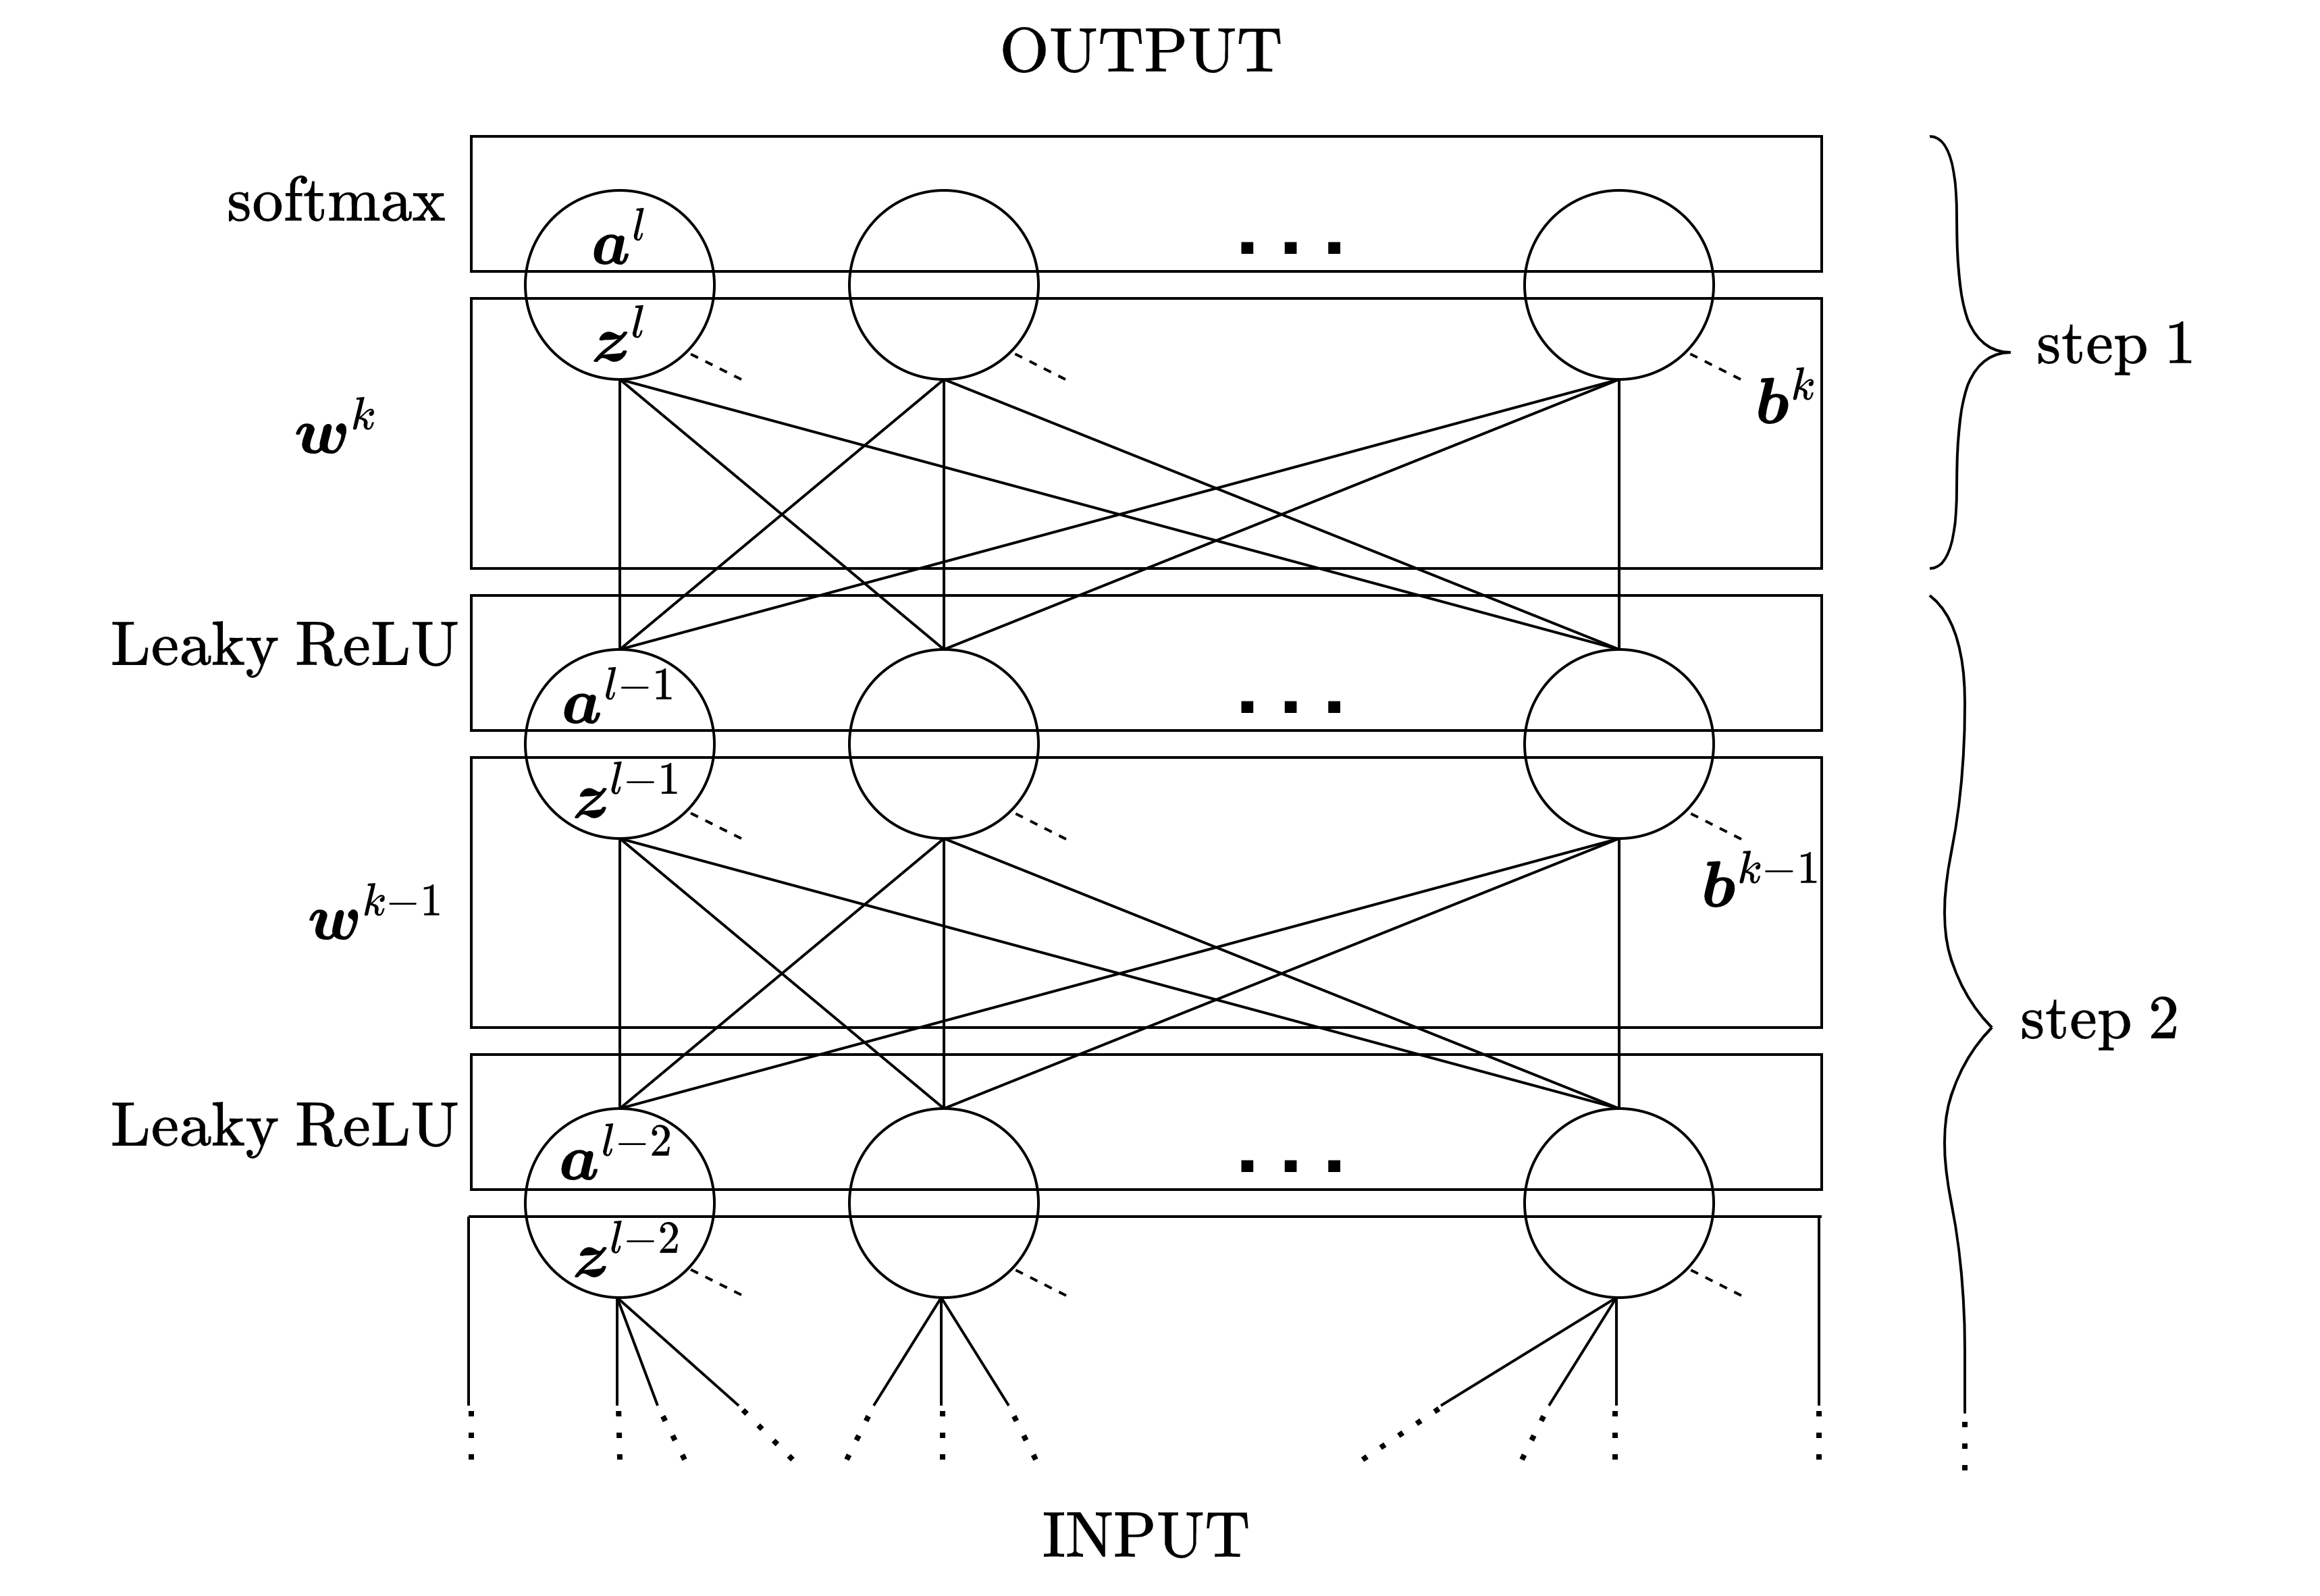
\includegraphics[width=0.8\textwidth]
    {images/neural_network.png}
    \caption{Illustration of a general feed-forward neural 
    network}
    \label{fig:neural_net_backprop}
\end{figure}


\subsubsection{Predicting}

Predicting in a feed-forward neural network is done by performing 
a forward pass. As mentioned earlier, a forward pass is, as the 
name suggests, the data points passing through the network, and 
one by one the weighted sum is computed together with the weights 
and biases. The weighted sum is then passed through the given 
activation function, and the process is then repeated until the 
last layer is reached. 
In the last layer the five outputs are 
passed through the softmax activation function and a prediction 
is made to the class with the highest probability.


\subsubsection{Evaluating Correctness}

A neural network aims at approximating a function that can map 
attributes to an output, and is rather good at it. Even simple 
networks can approximate any continuous function with reasonable 
accuracy.
We constructed a reference implementation from the keras API 
\autocite{chollet2015keras} of the TensorFlow library, yielding a 
accuracy of $73\%$ with the same parameters as our own model. 
But using a reference implementation to compare to our own 
implementation is not informative enough, because it is difficult 
to reproduce the exact same model. Therefore we decided to 
look at other methods to evaluate our model.

An essential indicator that an implementation is correct, is if 
the model is able to learn the patterns of the training set. 
That is, we train the model and obtain a reasonable accuracy. 
Because of the flexibility of the learning method, we also expect 
the model to be able to completely overfit the training data. 
Lastly, since we train the model using gradient descent, we 
expect the training accuracy to increase for each epoch, and the 
loss to decrease. 
We first evaluate our implementation, on two toy data sets 
checking if we are able to overfit the data i.e., obtaining a 
training accuracy close to $100\%$, using a simple network. We 
train the two data sets with their respective model both having 
one hidden layer with $20$ neurons. As expected, the two models 
were able to overfit their training data. 

Then we evaluate our implementation again on a stratified subset 
of $500$ samples of the given fashion MNIST training set. We 
train a simple network with $1$ hidden layer of $20$ neurons with 
Leaky ReLU as activation function and softmax as the output 
activation function. We used $30$ batches and $200$ epochs with a 
learning rate of $0.0001$. The loss history and training accuracy 
plotted against epochs is depicted in \autoref{fig:Train accuracy 
loss eval}.

\begin{figure}[ht]
    \centering
    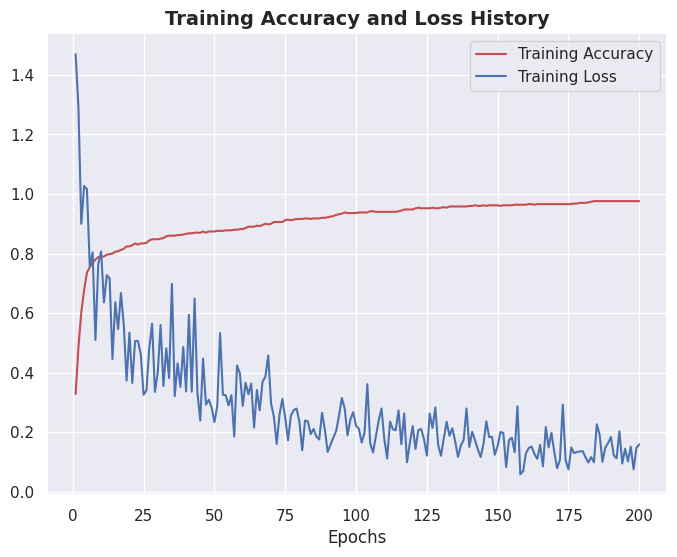
\includegraphics[width=0.5\textwidth]
    {ModelEval_acc_loss}
    \caption{Over fitting subset of training set with our own 
    implementation of the neural network}
    \label{fig:Train accuracy loss eval}
\end{figure}

It is clear that the model is able to overfit the training data 
and that the accuracy increases while the loss decreases. Notice 
that the loss does not decrease for each epoch, but is rather 
jagged because of the small batch size.
We can conclude that all the evaluations of the model indicate 
that the model has been implemented correctly and is in fact able 
to learn the patterns of the data it has been given. 


\end{document}